\documentclass[11pt]{scrartcl}

\usepackage{ucs}
\usepackage[utf8x]{inputenc}
\usepackage[T1]{fontenc}
\usepackage[ngerman]{babel}
\usepackage{amsmath,amssymb,amstext}
\usepackage{graphicx}
\usepackage[justification=RaggedRight, singlelinecheck=false]{caption}
\usepackage{tikz}
\usepackage[square,sort,comma,numbers]{natbib}
\usepackage{url}

\title{Fortgeschrittenen Praktikum Teil 1: IKF}
\subtitle{Versuch 2: Schnelle Neutronen \\ Betreuer: Philipp Sitzmann}

\author{Gruppe 1: Reinhold Kaiser, Florian Stoll}

\date{07.05.2018}

\begin{document}
\maketitle
\newpage
\tableofcontents
\newpage
\bibliographystyle{alphadin}
\section{Zielsetzung}
\section{Theoretische Grundlagen}

\subsection{Neutronenstrahlung}
Neutronen tragen keine Ladung und auch ihr magnetisches Moment ist so gering, dass es in diesem Versuch vernachlässigt werden kann, sodass keine elektromagnetische Wechselwirkung zwischen Neutronen und Elektronen vorhanden ist. Neutronen geben ihre Energie daher ausschließlich über die starke Wechselwirkung an die Kerne ab. Dabei kann der Stoßprozess mit Hilfe  klassischer Mechanik beschrieben werden. Der Wirkungsquerschnitt hängt  dabei aber von der Masse des Stoßpartners und der Energie des Neutrons ab \cite{anleitung}.
Um nun die Neutronen zu detektieren werden große Detektoren benötigt, da Wirkungsquerschnitt im Allgemeinen sehr klein ist. Dort wird dann ausgenutzt, dass die Wasserstoffkerne, an denen die Neutronen streuen, im Szintillator registriert werden können. So kann das Proton mit den Elektronen wechselwirken, die dann ein Signal erzeugen, dass proportianal zur Elektronenenergie ist. Allerdings ist die vom Neutron an das Proton abgegebene Energie abhängig vom Rückstoßwinkel $\Phi$, des Stoßprozesses:
\begin{equation}
 E_R = \frac{4A}{(A+1)^2}E_n\cos^2\Phi
\end{equation}
Dabei ist $A$ die Massenzahl des Stoßpartners und $E_n$ die Neutronenenrgie. Für ein Proton ($A=1$) ist die maximale Energie $E_n$ im Falle eines zentralen Stoßes und $0$ im Falle eines Streifschusses. Die Energieverteilung ist also kontinuierlich, die maximal gemessene Energie entspricht aber der Energie der Neutronen.

\subsection{Wechselwirkung von $\gamma$-Strahlung mit Materie}
Im Wesentlichen wechselwirken $\gamma$-Quanten mit Materie auf fünf unterschiedliche Arten: elastische Streuung, Compton-Streuung, Photoeffekt, Mößbauer-Effekt und Paarbildung. In diesem Versuch sind aber nur die Compton-Streuung und der Phtoeffekt von Relevanz, weswegen wir uns hier im Protokoll darauf beschränken.
\subsubsection{Compton-Streuung}
Trifft ein Photon auf ein schwach gebundenes Elektron eines Atoms, so wird durch einen elastischen Stoß ein Teil seines Impulses und seiner Energie auf dieses Elektron übertragen. Das Elektron verlässt das Atom, während das gestreute Photon an Energie verliert. Der Energieverlust des gestreuten Photons führt zu einer Frequenzänderung. Je nach Streuwinkel $\theta$ verändert sich dieser Energieübertrag an das Elektron.
\begin{equation}
 E=\frac{\alpha(1-\cos \theta)E_\gamma}{1+\alpha(1-\cos\theta)},
\end{equation}
dabei ist $\alpha=\frac{E_\gamma}{m_e\cdot c^2}$ und $E_\gamma$ die Energie des Gammaquants. Das Maximum wird bei einem Winkel von $180\circ $ erreicht, wodurch sich die Formel zu
\begin{equation}
 E_{max}=\frac{2\alpha E_\gamma}{1+2\alpha}
\end{equation}
reduziert. An diesen Stellen treten im Spektrum die Comptonkanten auf, da von Gammaquanten mit einer bestimmten Energie $E_\gamma$ keine Elektronen induziert werden, die eine höhere Energie haben.


Der Wirkungsquerschnitt der Compton-Streuung an einem bestimmten Material steigt dabei mit zunehmender Kernladungszahl und nimmt mit steigender Photonenenergie ab. 
\subsubsection{Photoeffekt}
Beim Photoeffekt wird ein Photon von einem Hüllenelektron absorbiert. Es kommt zum vollständigen Energieübertrag an das Elektron, wodurch es aus seiner Bindung mit dem Atomkern gelöst wird und das Atom verlässt. Damit dieser Vorgang stattfinden kann, muss die Energie $E_\gamma$ des einfallenden Photons größer sein als die Bindungsenergie $E_b$ des Elektrons. Je nachdem, in welcher Elektronenschale sich das Elektron befindet, variiert diese Bindungsenergie. Wegen der Impulserhaltung werden bevorzugt Elektronen aus den beiden innersten Schalen herausgelöst. Die kinetische Energie des emitierten Eletrkons folgt dabei der Beziehung
\begin{equation}
E_{kin}=E_\gamma - E_b
\end{equation}
Da nun in einer der energetisch niedrigeren Schalen ein Elektron fehlt, tritt an dessen Stelle ein Elektron aus einem energetisch höheren Niveau. Die dabei freiwerdende Energie wird in Form eines charakteristischen Photons abgestrahlt.

\subsection{$^{241}$Am-$^9$Be-Neutronenquelle}
Americium-241 zerfällt unter Aussendung eines Alpha-Teilchens zu Neptunium-237. Das Alpha-Teilchen hat dabei eine Energie von ungefähr $5,5MeV$ \cite{americium}, wodurch es die Kernreaktion
\begin{equation}
 ^4\alpha + \,^9Be \rightarrow\, ^{12}C +\, ^1n
\end{equation}
induzieren kann.

\begin{figure}[htbp]  
     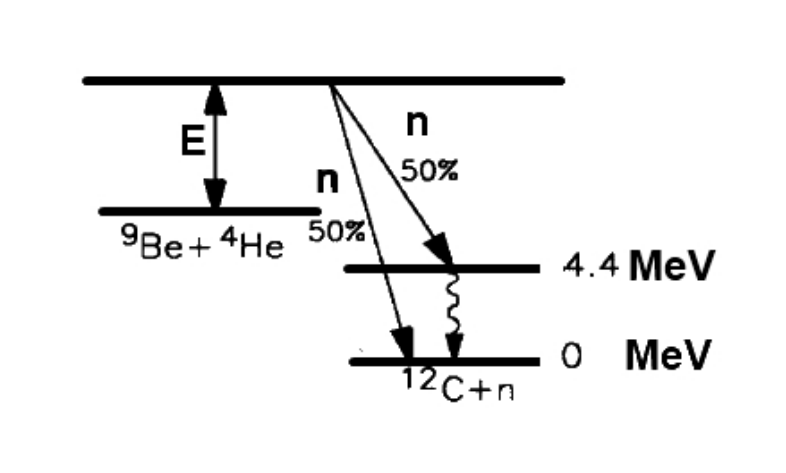
\includegraphics[width=0.7\textwidth]{beryllium.png}
  \caption{Energieschema für den Alpha-Teilcheneinfang von $^9$Be \cite{anleitung}}
  \label{beryllium}
\end{figure}

Wie in Abbildung \ref{beryllium} zu erkennen ist, zerfällt der
angeregte Zustand von $^13$C zu jeweils $50\%$ über zwei unterschiedliche Wege. Die angeregten Zustände zerfallen aber direkt bei einer sehr kurzen Lebensdauer zum $^{12}$C-Grundzustand, wobei bei der Kaskade auch ein $\gamma$-Quant ausgesendet wird.

\subsection{$^{22}$Na-Gammastrahlenquelle}
Diese Gammastrahlenquelle wird zur Energiekalibrierung verwendet, da $^{22}$Na über einen energetisch klar definierten kurzlebigen Zwischenzustand zerfällt (siehe Abbildung \ref{na22}).

\begin{figure}[htbp]  
     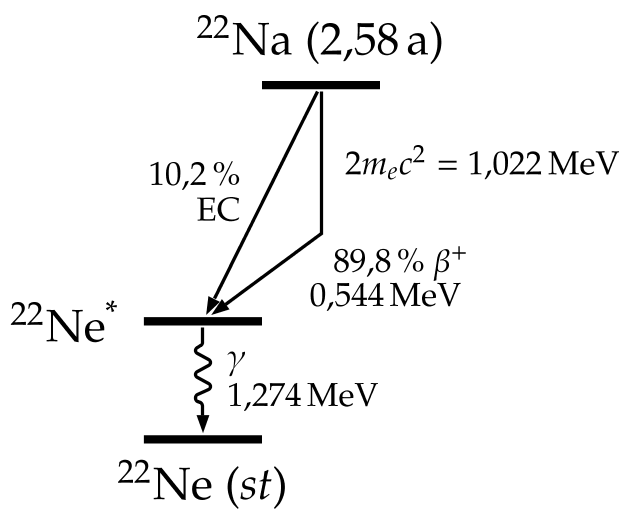
\includegraphics[width=0.6\textwidth]{Na22.png}
  \caption{Energieschema für den Zerfall von $^{22}$Na zu $^{22}$Ne \cite{na22}}
  \label{na22}
\end{figure}

Zunächst wird ein Positron ausgesendet, welches ein Ruhemasse von $511keV$ hat. Der angeregte Zustand $^{22}$Ne zerfällt dann unter Aussendung eines Gammaquants mit der Energie $1274keV$ zum Grundzustand von $^{22}$Ne. Zusätzlich zu dem klar definierten Gammaquant entstehen bei der Annihilation des Positrons mit einem Elektron des umgebenden Materials zwei weitere Gammaquanten, die beide die Energie $511keV$ haben.

\subsection{Organische Szintillatoren}
\begin{figure}[htbp]  
     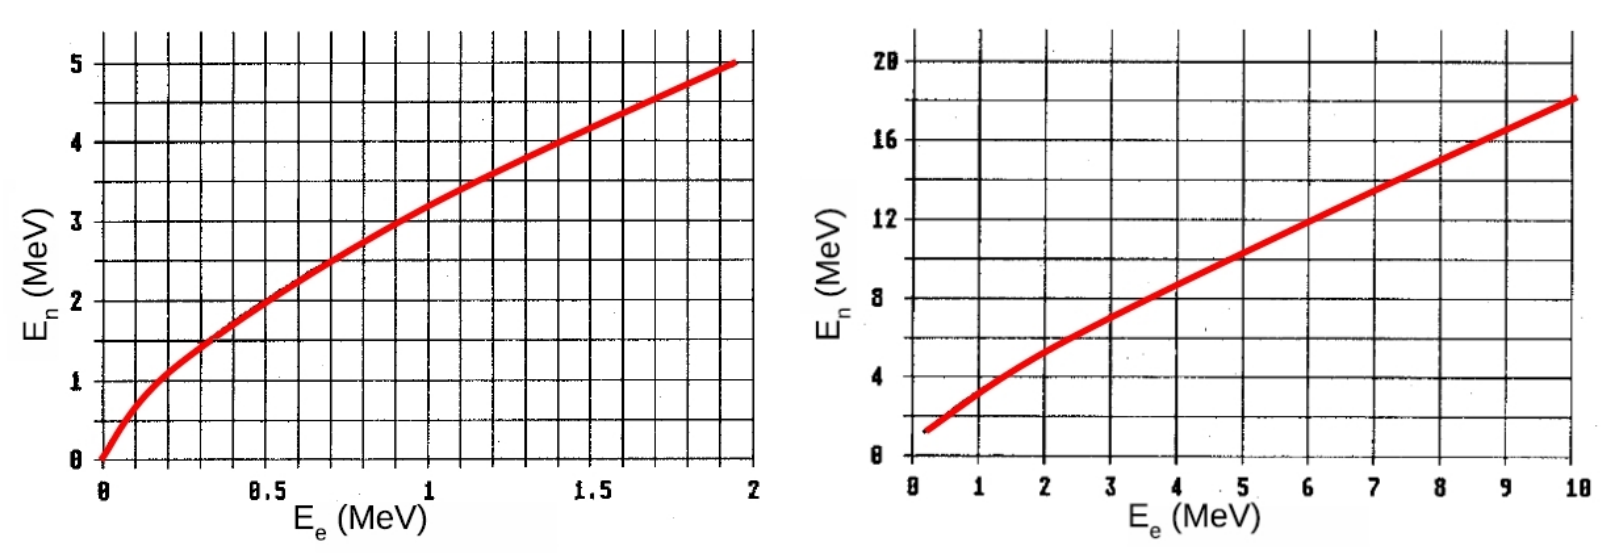
\includegraphics[width=0.7\textwidth]{szintillator.png}
  \caption{Zusammenhang zwischen Neutronen- und Elektronen-Energien beim NE213 \cite{anleitung}}
  \label{szintillator}
\end{figure}
Organische Szintillatoren haben einige Eigenschaften, die sie zu guten Detektoren für die Detektion von Gammaquanten und Neutronen machen. Der hohe Wasserstoffgehalt führt dazu, dass der Protonen-Neutronen-Stoß für den Nachweis der Neutronen und ihrer Energie heranagezogen werden kann. Außerdem besitzen organische Szintillatoren sehr kurze und teilchenspezifische Abklingzeiten, was zum einen Zeitmessungen und hohe Zählraten zulässt. Zum anderen kann eine Unterscheidung der Teilchen durch Pulsformdiskriminierung stattfinden. Somit können solche Detektoren auch zur Neutronendetektion bei starkem Gamma-Hintergrund benutzt werden, obwohl sie auch eine sehr hohe Ansprechwahrscheinlichkeit für Gammaquanten haben.

Da die Kalibrierung mit Hilfe des Comptoneffekts stattfindet, sind die gemessenen Energien im Detektor Elektronenenergien. Um nun auf die Neutronenenergien zu kommen, gibt es empirisch bestimmte Zusammenhangskurven, die in Abbildung \ref{szintillator} zu sehen sind. So muss nach der Kalibrierung die Energie der Neutronen mithilfe dieser Kurven ungefähr abgelesen werden.

\subsection{Pulsformdiskriminierung}
Um in der Zählrate des organischen Szintillators zwischen den Gammaquanten und Neutronen zu unterscheiden, macht man sich zu Nutze, dass die Pulsform für Neutronen und Gammaquanten unterschiedlich ist. Dies hängt mit der spezifischen Energieabgabe der einzelnen Teilchen im Szintillatormaterial zusammen. 

Mit Hilfe einer geeigneten elektrischen Schaltung wird so eine Pulsformdiskriminierung (PSD) zwischen Neutronen und Gammaquanten erreicht. Im Prinzip funktiert dies so, dass das aufintegrierte Signal mehrfach invertiert und verzögert aufsummiert wird. Durch die unterschiedlichen Antiegszeiten der Signale wird erreicht, dass das resultierende Signal unterschiedliche Nulldurchgänge hat. Aus dieser bestimmten Zeit wird dann das für Neutronen und Gammaquanten charakteristische PSD-Signal gewonnen. Trägt man dieses Signal über der Energie der Teilchen auf, gelingt es gut, die für die Messung gewünschten Teilchen auszuwählen.




\section{Versuchsaufbau und Messgeräte}

\begin{figure}[htbp]  
     \usetikzlibrary{shapes,arrows}
\tikzstyle{block} = [draw, fill=blue!20, rectangle, 
    minimum height=3em, minimum width=4em]
\tikzstyle{circle} = [draw, fill=blue!20, ellipse, 
    minimum height=2.5em, minimum width=2.5em]
\begin{tikzpicture}
 \coordinate (L) at (-5,0);
 \coordinate (R) at (5,0);
\coordinate (A) at (2.5,4.3);
\coordinate (O) at (2.5,0);

\draw[dash pattern=on5pt off3pt] (L) -- (R);


\node[block, name=det1] at (L) {Det1};
\node[block, name=det2, rotate=0] at (R) {Det2};
\node[circle, name=source] at (O) {Q};

\end{tikzpicture}
  \caption{Schematischer Aufbau zur Energie-Kalibrierung mit der Quelle (Q) $^{22}$Na}
  \label{aufbau1}
\end{figure}

In diesem Versuch werden zwei Detektoren vom Typ NE213 verwendet. Zunächst wird eine Natrium-22-Quelle in der Mitte dieser beiden aufeinander gereichteten Detektoren platziert (siehe Abbildung \ref{aufbau1}). Nach der Kalibrierung wird nun diese Quelle mit einer Americium-241-Berillium-9-Quelle ausgetauscht. Die Absorber, die nun in den Strahlengang zwischen der Quelle und dem Detektor 1 gestellt werden, müssen einen bestimmten Abstand $a$ zu dem Detektor haben (siehe Abbildung \ref{aufbau2}). Die Bedingung dafür ist, dass die Neutronenstrahlen von der Quelle Q (als punktförmig angenommen) die gesamte Länge $l$ des Absorbers durchqueren  müssen, bevor sie den Detektor erreichen. Detektoren und Absorber sind zylinderförmig und die Zylinderachse liegt auf der Strahachse. Aus dem Strahlensatz ergibt sich dann mit dem Abstand Quelle - Detektor $x$, Durchmesser Detektor $D$ und Durchmesser Absorber $d$
\begin{equation}
 \frac{x-a}{d} = \frac{x}{D}
\end{equation}
und dann auch direkt 
\begin{equation}
 a = x\left(1-\frac{d}{D}\right).
\end{equation}

\begin{figure}[htbp]  
     \usetikzlibrary{shapes,arrows}
\tikzstyle{ann} = [fill=white,font=\footnotesize,inner sep=1pt]
\tikzstyle{block} = [draw, fill=blue!20, rectangle, 
    minimum height=2.5em, minimum width=3em]
\tikzstyle{circle} = [draw, fill=blue!20, ellipse, 
    minimum height=0.75em, minimum width=0.75em]
\begin{tikzpicture}
 \coordinate (L) at (-5,0);
 \coordinate (R) at (5,0);
\coordinate (A) at (2.5,4.3);
\coordinate (O) at (2.5,0);

\draw[dash pattern=on5pt off3pt] (L) -- (R);


\node[block, name=det1, minimum height=5em, minimum width=7em] at (L) {Det1};
\node[block, name=det2, minimum height=5em, minimum width=7em, rotate=0] at (R) {Det2};
\node[circle, name=source] at (O) {};
\node[block, name=absorber] at (-0,0){Abs.};

\draw[dash pattern=on5pt off3pt] (O) -- (-3.6,1);
\draw[dash pattern=on5pt off3pt] (O) -- (-3.6,-1);

\draw[arrows=<->](-3.75,1)--(-3.75,-1);
\node[ann] at (-3.75,0) {$D$};

\draw[arrows=<->](-3.5,-1.5)--(-0.6,-1.5);
\node[ann] at (-2.05,-1.5) {$a$};

\draw[arrows=<->](0.6,-1.5)--(-0.6,-1.5);
\node[ann] at (0,-1.5) {$l$};

\draw[arrows=<->](0.6,-1.5)--(2.5,-1.5);
\node[ann] at (1.55,-1.5) {$b$};

\draw[arrows=<->](-0.8,-0.5)--(-0.8,0.5);
\node[ann] at (-0.8,0) {$d$};

\draw[arrows=<->](-3.5,1.5)--(2.5,1.5);
\node[ann] at (-0.5,1.5) {$x$};

\draw[arrows=<->](3.5,1.5)--(2.5,1.5);
\node[ann] at (3,1.5) {$y$};

\node[ann] at (2.5,0.4) {Q};




\end{tikzpicture}
  \caption{Schematischer Aufbau zur Kernradienbestimmung des Absorbers (Abs.) mit der Quelle (Q) $^{241}$Am-$^9$Be}
  \label{aufbau2}
\end{figure}

Mit den Werten $D=11,43 cm$, $d= 4cm$ und $x=50cm$ erhält man $a=32,5 cm$. Da die Länge dea Absorbers $l=5cm$ ist, erhält man für $b=12,5cm$. Für die Time-of-Flight-Messung ist es noch wichtig $y=3,15cm$ zu wissen.

Die Signale aus den Detektoren werden über eine Verstärkerelektronik und einen Analag-Digital-Wandler zum Computer geführt, auf dem die Signale dargestellt werden. Außerdem gibt es einen Zeit-Analysator der Koinzidenzen zwischen den beiden Detektoren erkennt und Zeitdifferenz auf dem Computer darstellt. Als letztes ist das PSD-Signal zu nennen, was in der Elektronik generiert wird und auf dem Computer als 2D-Histogramm dargestellt werden kann.

\section{Kalibrierung}

\subsection{Energie}


\subsection{Time of Flight}
\section{Durchführung und Auswertung}

\subsection{Kernradienbestimmung}

Mithilfe der Am-Be-Neutronenquelle sollen im eigentlichen Versuchsteil nun die Kernradien verschiedener Absorbermaterialien bestimmt werden. 
Dafür benötigt man den totalen Wirkungsquerschnitt der Reaktion der Neutronen im Absorber. Diesen kann man über die verschiedenen Zählraten der eingesetzten Absorber wie folgt bestimmen:

\begin{align}
Z=Z_=\cdot e^{-\mu d}
\end{align}

Dabei entspricht Z der Zählrate mit Absorber, $Z_0$ der Zählrate ohne Absorber, d der Dicke des Absorber und $\mu$ dem sogenannten Schwächungskoeffzienten, welcher wie folgt mit dem totalen Wirkungsquerschnitt $\sigma_{tot} = 2\pi R^2$ und der Zahl der Kerne pro $cm^3$ N zusammenhängt:

\begin{align}
\mu=\sigma_{tot}\cdot N 
\end{align}

Über die verschiedenen Zählraten können so $\mu$, $\sigma_{tot}$ und damit R bestimmt werden. Die bestimmten Werte können anschließend zur Bestimmung der Radiuskonstante $r_0$ verwendet werden, da folgende Beziehung gilt:

\begin{align}
R=r_0 \cdot A^{1/3}
\end{align}

Da das Neutron weiterhin nur bis auf eine reduzierte De-Broglie-Wellenlänge lokalisiert werden kann, ergibt sich die reduzierte De-Broglie-Wellenlänge $\lambda_{dB}$ als Offset der gerade genannten Beziehung.

Für die Messung werden die verschiedenen Absorber in die in Abschnitt 3 bestimmte Position gebracht und die entsprechenden Spektren mit einer Messdauer von 1920s vermessen. Weiterhin werden nur Neutronen mit einer Energie von über 7MeV als "richtige" Neutronen angenommen, da der oben angenommene Wirkungsquerschnitt nur in diesem Energiebereich gültig ist. Dafür muss bei der Bestimmung der Zählrate der richtige Bereich des 2D-Histogramms ausgewählt werden, wobei hier nur 128 Kanäle vorhanden sind. Über die oben schon dargestellte Energierelation zwischen Neutronen und Elektronen, kann eine minimale Elektron-Energie von 3MeV identifiziert werden. Im schon kalibrierten Energie-Diagramm mit 2014 Kanälen entspricht dies allen Ereignissen ab Kanal 562. Umgerechnet auf 128 Kanäle müssen wir also alle Neutronen-Ereignisse ab Kanal 71 zählen, um auf die korrekte Zählrate zu kommen. Die bei den verschiedenen Absorbern aufgenommenen Zählraten gemeinsam mit den Atommassen und Dichten der Absorbermaterialien finden sich in \ref{werte}. 

\begin{table}[h]
	\caption{Neutronen-Zählraten mit verschiedenen Absorbermaterialien}
	\begin{tabular}{|c|c|c|c|c|c|c|c|c|}
	\hline
	 Absorber & Zählrate & Atommasse in u & Dichte in g/$cm^3$ & Teilchen / $cm^3$ & $\mu$ & $\sigma$ & R & $A^\frac{1}{3}$ \\ \hline
	  ohne & 23713 &  &  &  &  & &  &   \\ \hline
	   Cadmium & 10785 & 112,4 & 8,65 & $4,63 \cdot 10^{22}$ & 0,157 & $3,4\cdot 10^{-24}$ & $7,36 \cdot 10^{-13}$ & 4,83\\ \hline
	    Aluminium & 13459 & 27 & 2,69 & $5,99 \cdot 10^{22}$ & 0,113 & $3,4\cdot 10^{-24}$ & $5,48 \cdot 10^{-13}$  & 3 \\ \hline
	     Blei & 10714 & 207 & 11,3 & $3,28 \cdot 10^{22}$ & 0,159 & $3,4\cdot 10^{-24}$ & $8,77 \cdot 10^{-13}$  & 5,92 \\ \hline
	      Eisen & 7434 & 55,8 & 7,87 & $8,49 \cdot 10^{22}$ & 0,232 & $3,4\cdot 10^{-24}$ & $6,59 \cdot 10^{-13}$  & 3,82 \\ \hline
	       Kupfer & 6990 & 63,5 & 8,92 & $8,45 \cdot 10^{22}$ & 0,244 & $3,4\cdot 10^{-24}$ & $6,78 \cdot 10^{-13}$  & 3,99\\ \hline
	\end{tabular}
\label{werte}
\end{table}

Die bestimmten Werte für R können gegenüber der dritten Wurzel der Massenzahl aufgetragen und aus der Steigung die Radiuskonstante $r_0$ und aus dem y-Achsenabschnitt die De-Broglie-Wellenlänge bestimmt werden. In Abbildung \ref{kernradien} findet sich dieser Plot. Als fehlerbehaftete Größen wurden die Dicke der Absorber und die Zählraten angenommen, wobei der Fehler der Absorberdicke auf $\Delta d = 1mm$ geschätzt wurde, während die Zählraten als normalverteilte Größen und damit mit einem Fehler von $\sqrt{Z}$ behaftet angenommen wurden. Der Fehler für R ergibt sich dann zu:
\begin{align} 
\Delta R = R \left(\frac{\Delta d}{2d}\right) + \frac{\Delta Z_0}{2Z_0\log\frac{Z_0}{Z}}+\frac{\Delta Z}{2Z\log\frac{Z_0}{Z}}
\end{align}

\begin{figure}[htbp]  
     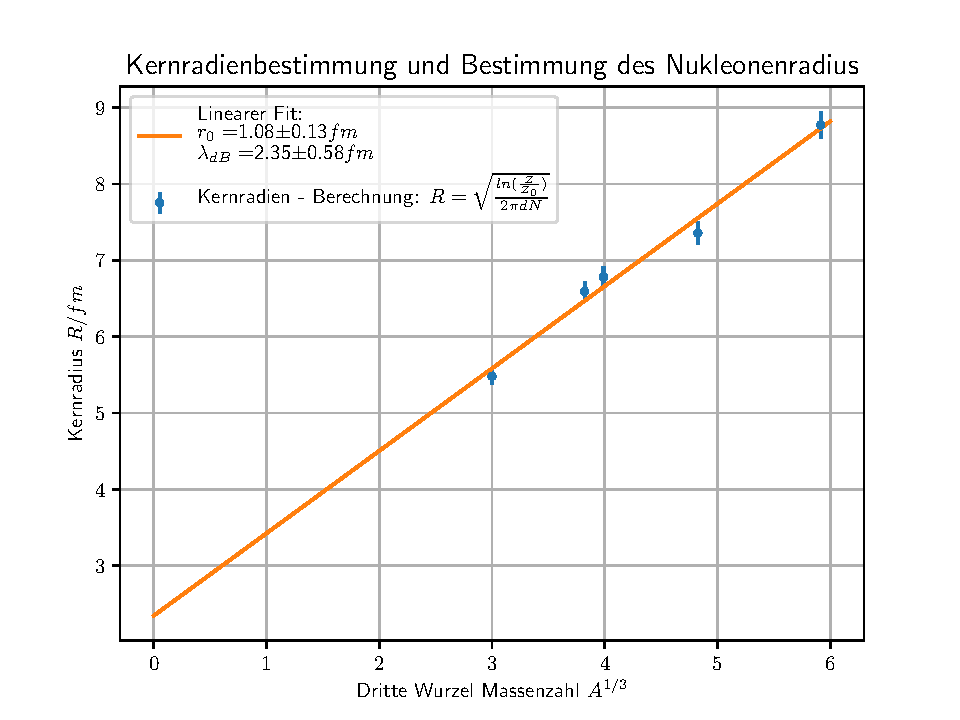
\includegraphics{kernradien.pdf}
  \caption{Kernradien über der dritten Wurzel der Massenzahl}
  \label{kernradien}
\end{figure}

Als Ergebnis finden wir so eine Radiuskonstante von $r_0=1,08 \pm 0,13 fm$. Der Literaturwert beträgt hier $\approx 1,2 fm$, unsere Messung ergibt also innerhalb der Fehlergrenzen einen absolut plausiblen und guten Wert. Unser Wert für die De-Broglie-Wellenlänge beträgt für die Neutronen $\lambda_{dB}=2,35 \pm 0,58 fm$. Über die relativistische Energie-Impuls-Beziehung und die Definition der De-Broglie-Wellenlänge lässt sich daraus eine Neutronenenergie von 526 MeV ableiten. Dieser Wert erscheint jedoch sehr unrealistisch, da die typischen Neutronenenergien der verwendeten Quelle im 1-10MeV - Bereich liegen. Als mögliche Fehlerquellen sind hier auf jeden Fall die einfache Abschätzung des Wirkungsquerschnitts und die geometrischen Fehler der Absorber zu nennen.

\subsection{Time of Flight - Messung}

Für die Time-of-Flight-Messung wird aus den Daten der Messung der Kernradienbestimmung ohne Absorber die Lage der Peaks bestimmt. Die Abstände der beiden Detektoren zur Quelle betragen dabei einmal 50cm und einmal 3,15 cm. Im ToF-Spektrum treten dabei insgesamt 4 Peaks auf, welche aus den verschiedenen Kombinationen der Ansprechmöglichkeiten der beiden Detektoren resultieren. So kann ein bei der Kernreaktion entstehendes Neutron entweder im ersten oder im zweiten Detektor registriert werden, während der jeweils andere eines der entstehenden Photonen registrieren kann. Aus den unterschiedlichen Flugzeiten der Neutronen entstehen so die verschiedenen Peaks.

Die energiereichsten Neutronen sind im Spektrum durch den Peak mit der geringsten Zeitdifferenz zu finden. Über die Kanallage bei Kanal 493 und der geometrischen Abmessung des Aufbaus ergibt sich mit der vorausgegangenen Eichung eine kinetische Energie von 3,29 MeV für die Neutronen. Über das im Theorieteil gezeigte Zerfallsschema, wäre eigentlich eine Maximalenergie von 4,4 MeV zu erwarten gewesen, da die zu 50\% entstehende Zwischenstufe noch genau diese Anregungsenergie aufweist. Im Rahmen der vorliegenden Fehlerquellen (keine punktförmige Quelle, ungenaue Peakbestimmung, fehlerhafte Elektronik) ergibt unsere Messung jedoch eine gute Größenordnung. Die Neutronen besitzen mit dieser Energie ungefähr 10\% der Lichtgeschwindigkeit, sodass auch relativistische Effekte durchaus eine Begründung für die Abweichung darstellen. 

\section{Zusammenfassung/Fazit}

\bibliography{Literaturverzeichnis}



\end{document}
